\chapter{Analiză și proiectare}

\section{Scenarii de utilizare}

Utilizatorul poate efectua următoarele acțiuni:
\subsection{Logare}
Utilizatorul se loghează în aplicație, care îl va redirecta către platforma Flickr, pentru a efectua autentificarea prin intermediul acesteia.

\subsection{Alege sursa imaginilor}
Utilizatorul poate alege sursa imaginilor ce vor fi analizare: propriul profil, imaginile contactelor sale, sau imagini publice de pe platforma Flickr.

\subsection{Încarcă imagine}
Pentru a efectua această acțiune, utilizatorul trebuie să fi trecut prin pasul de logare și eventual să fi ales sursa imaginilor. Dacă acesta nu a ales sursa imaginilor, în mod implicit aceasta este propriul profil. Scenariul acesta de utilizare presupune ca utilizatorul să aleagă o imagine de pe propriul dispozitiv pe care să o trimită către aplicație.

Pentru a returna imaginile similare din punct de vedere vizual, aplicația va efectua următoarele acțiuni:
\begin{enumerate}
    \item Analizează imaginea încărcată folosind o rețea neurală și returnează o serie de etichete descriptive
    \item Aduce imaginile  din sursa selectată de utilizator
    \item Analizează imaginile aduse, obținând pentru fiecare o serie de etichete
    \item Descoperă similaritatea între imagini comparând etichetele și obține o listă de imagini corespunzătoare
    \item Afișează imaginile din lista obținută
\end{enumerate}{}

 \begin{figure}[!htbp]
    \begin{center}
        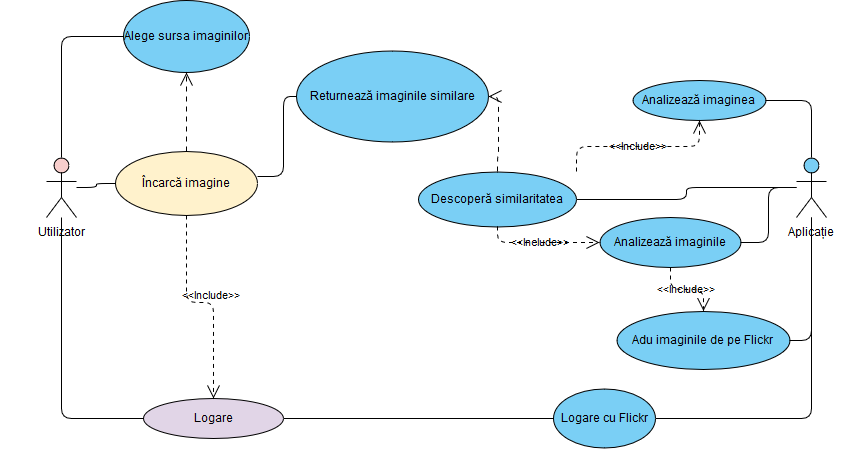
\includegraphics[width=0.9\textwidth]{images/use_case.png}
        \caption{Diagrama de scenarii de utilizare a aplicației}
    \end{center}
\end{figure}


\section{Arhitectura aplicației}
Aplicația este împărțită în două module, dar folosește și anumite servicii externe.Utilizatorul interacționează direct cu modulul  \textit{front-end}, o aplicație web realizată cu ajutorul \textit{framework}-ului Angular în limbajul Typescript. La rândul său, modulul este împărțit în mai multe componente, acestea apelând unele servicii. Modulul de back-end este realizat cu ajutorul \textit{framework}-ului Flask în limbajul Python. Se folosesc mai multe biblioteci pentru a efectua anumite operații(ex. \textit{requests} pentru a apela API-uri, \textit{pony.orm} pentru conectarea la baza de date) și \textit{framework}-uri specializate pentru rețele neuronale(Tensorflow și Keras). Serviciile externe sunt reprezentate de API-urile platformelor Flickr(pentru autentificare, informații despre profil și imagini) și DataMuse(pentru a obține sinonime). De asemenea se mai folosește o bază de date SQLite pentru reținerea \textit{token}-ului de acces și identificatorului unic.

 \begin{figure}[!htbp]
    \begin{center}
        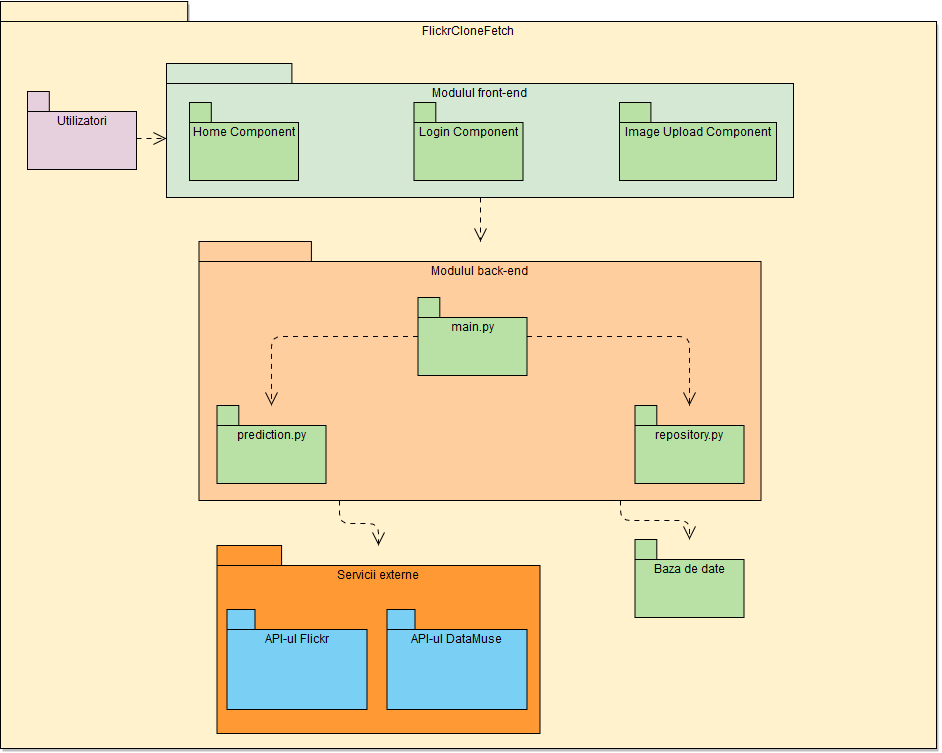
\includegraphics[width=1.0\textwidth]{images/arhitectura.png}
        \caption{Arhitectura aplicației}
    \end{center}
\end{figure}

\section{Planificarea activităților realizate de către aplicație}
Fluxul de activități în cadrul aplicației se desfășoară în modul urmator
\begin{enumerate}
    \item Modulul \textit{front-end} afișează pagina de logare și redirectează utilizatorul la procesul de logare de pe \textit{back-end} (Home Component)
    \item Modulul \textit{back-end} trimite cererea de logare prin OAuth la API-ul Flickr
    \item  Se salvează \textit{request token}-ului și redirectarea la autorizarea OAuth prin API-ul Flickr
    \item  Se generează un identificator unic pentru utilizator, se salvează în baza de date împreună cu \textit{token}-ul de acces primit și apoi se face redirectarea către \textit{front-end} trimițând și identificatorul unic
    \item Modulul \textit{front-end} reține identificatorul utilizatorului și cere  datele despre profil 
    \item Modulul \textit{back-end} furnizează datele despre profil(nume utilizator, imagine de profil)
    \item \textit{Front-end}-ul redirectează utilizatorul la pagina de încărcare imagini (Login Component)
    \item Aici i se oferă utilizatorului posibilitatea de a încărca o imagine și de a alege sursa imaginilor, apoi trimite la modulul \textit{back-end} aceste informații (Image Upload Component)
    \item Modulul \textit{back-end} primește imaginea și opțiunile privitoare la sursă și  analizează imaginea cu o rețea neurală, obținând o listă de etichete
    \item Se apelează API-ul DataMuse pentru a obține cuvinte similare etichetelor obținute
    \item Se apelează API-ul Flickr pentru a obține imagini și acestea se  analizează cu rețeaua neurală
    \item Se compară etichetele imaginilor cu etichetele imaginii încărcate și se creează o listă de imagini similare
    \item Se returnează lista către \textit{front-end}
    \item \textit{Front-end}-ul afișează imaginile returnate de \textit{back-end} (Image Upload Component)
\end{enumerate}{}


